\documentclass[11pt]{article}

% Change "review" to "final" to generate the final (sometimes called camera-ready) version.
% Change to "preprint" to generate a non-anonymous version with page numbers.
\PassOptionsToPackage{numbers}{natbib}
\usepackage[preprint]{acl}
%\usepackage[square,numbers]{natbib}


% Standard package includes
\usepackage{times}
\usepackage{latexsym}

% For proper rendering and hyphenation of words containing Latin characters (including in bib files)
\usepackage[T1]{fontenc}
% For Vietnamese characters
% \usepackage[T5]{fontenc}
% See https://www.latex-project.org/help/documentation/encguide.pdf for other character sets

% This assumes your files are encoded as UTF8
\usepackage[utf8]{inputenc}

% This is not strictly necessary, and may be commented out,
% but it will improve the layout of the manuscript,
% and will typically save some space.
\usepackage{microtype}

% This is also not strictly necessary, and may be commented out.
% However, it will improve the aesthetics of text in
% the typewriter font.
\usepackage{inconsolata}

%Including images in your LaTeX document requires adding
%additional package(s)
\usepackage{graphicx}



\usepackage{hyperref}       % hyperlinks
\usepackage{url}            % simple URL typesetting
\usepackage{booktabs}       % professional-quality tables
\usepackage{amsfonts}       % blackboard math symbols
\usepackage{amsmath}       
\usepackage{nicefrac}       % compact symbols for 1/2, etc.
\usepackage{microtype}      % microtypography
\usepackage{xcolor}         % colors


\usepackage[inline]{enumitem}
\usepackage{makecell}
\usepackage{fancyhdr}       % header
\usepackage{subcaption}
\usepackage{mdframed}
\usepackage{comment}
\usepackage{tabularx}
\usepackage{caption}
\usepackage{placeins}
\usepackage{float}
\usepackage{array} % for centering column content  
\usepackage{wrapfig}
\usepackage{cleveref}
\usepackage{multirow}
\usepackage{algorithm}
\usepackage{algorithmic}
\usepackage{listings}
\usepackage{atbeginend}
%\usepackage{pifont}
\usepackage{csquotes} % Context-sensitive quotation marks 
\MakeOuterQuote{"}
\usepackage{lipsum}

\newenvironment{packed_enum}{
\begin{enumerate}
	\setlength{\itemsep}{1pt}
	\setlength{\parskip}{0pt}
	\setlength{\parsep}{0pt}
}{\end{enumerate}}

\newenvironment{packed_item}{
\begin{itemize}
	\setlength{\itemsep}{1pt}
	\setlength{\parskip}{0pt}
	\setlength{\parsep}{0pt}
}{\end{itemize}}

\newenvironment{packed_description}{
\begin{description}
	\setlength{\itemsep}{1pt}
	\setlength{\parskip}{0pt}
	\setlength{\parsep}{0pt}
}{\end{description}}

\AfterBegin{packed_enum}{\vspace{-0.7em}}
\AfterEnd{packed_enum}{\vspace{-0.7em}}
\AfterBegin{packed_item}{\vspace{-0.7em}}
\AfterEnd{packed_item}{\vspace{-0.7em}}
\AfterBegin{packed_description}{\vspace{-0.7em}}
\AfterEnd{packed_description}{\vspace{-0.7em}}

\AfterBegin{quote}{\vspace{-0.7em}}
\AfterEnd{quote}{\vspace{-0.7em}}

\lstdefinelanguage{json}{
basicstyle=\ttfamily,
numbers=left,
numberstyle=\tiny\color{gray},
stepnumber=1,
numbersep=8pt,
showstringspaces=false,
breaklines=true,
%	frame=lines,
%	backgroundcolor=\color{lightgray},
literate=
*{0}{{{\color{blue}0}}}{1}
{1}{{{\color{blue}1}}}{1}
{2}{{{\color{blue}2}}}{1}
{3}{{{\color{blue}3}}}{1}
{4}{{{\color{blue}4}}}{1}
{5}{{{\color{blue}5}}}{1}
{6}{{{\color{blue}6}}}{1}
{7}{{{\color{blue}7}}}{1}
{8}{{{\color{blue}8}}}{1}
{9}{{{\color{blue}9}}}{1}
{:}{{{\color{red}:}}}{1}
{,}{{{\color{red},}}}{1}
{\{}{{{\color{orange}\{}}}{1}
{\}}{{{\color{orange}\}}}}{1}
{[}{{{\color{orange}[}}}{1}
{]}{{{\color{orange}]}}}{1},
}

\lstdefinelanguage{txt}{
basicstyle=\ttfamily,
numbers=left,
numberstyle=\tiny\color{gray},
stepnumber=1,
numbersep=8pt,
showstringspaces=false,
breaklines=true,
%	frame=lines,
%	backgroundcolor=\color{lightgray},
}



%
% These are are recommended to typeset listings but not required. See the subsubsection on listing. Remove this block if you don't have listings in your paper.
\usepackage{newfloat}
%\DeclareCaptionStyle{ruled}{labelfont=normalfont,labelsep=colon,strut=off} % DO NOT CHANGE THIS
\lstset{%
basicstyle={\footnotesize\ttfamily},% footnotesize acceptable for monospace
numbers=left,numberstyle=\footnotesize,xleftmargin=2em,% show line numbers, remove this entire line if you don't want the numbers.
aboveskip=0pt,belowskip=0pt,%
showstringspaces=false,tabsize=2,breaklines=true}
\floatstyle{ruled}
\newfloat{listing}{tb}{lst}{}
\floatname{listing}{Listing}
%
% Keep the \pdfinfo as shown here. There's no need
% for you to add the /Title and /Author tags.
\pdfinfo{
/TemplateVersion (2024.1)
}

\setcounter{secnumdepth}{3} %May be changed to 1 or 2 if section numbers are desired.

%Header
\pagestyle{fancy}
\thispagestyle{empty}
\rhead{ \textit{ }} 

% Title

%\title{Evaluating LM Accuracy Uplift From Rewriting Questions to Remove Ambiguities}
%\title{Evaluating LM Accuracy Uplift: Using Answer Free Context to Double gpt-oss-20b Performance on a subset of HLE}
%\title{Evaluating LM Context Uplift: Doubling HLE Benchmark Performance Using Answer-Free Context}
%\title{LM Accuracy Uplift: Using Answer-Free Context Information to Double gpt-oss-20b Performance on a subset of HLE}
%\title{Squeezing All Improvement From Your Context: QA Accuracy Uplift Even When the Context Doens't Surface the Answer}
%\title{Evaluating LM Accuracy Uplift: Doubling the Performance on Humanity's Last Exam Using Answer-Free Context}
\title{Query Disambiguation via Answer-Free Context: Doubling Performance on Humanity’s Last Exam}




\author{%
Michael Majurski$^{12*}$ \quad Cynthia Matuszek$^{2}$\\
$^1$National Institute of Standards and Technology \quad $^2$University of Maryland Baltimore County\\
\texttt{michael.majurski@nist.gov}\\
\texttt{cmat@umbc.edu}\\
}





\begin{document}

\maketitle
% gpt-5-mini on HLE rewrite using gpt-oss-120b
% orig = 0.073
% rewrite = 0.439

% gpt-5-mini on HLE rewrite using gpt-oss-20b
% orig = 0.139
% rewrite = 0.372

\begin{abstract}
How eloquently, clearly, and unambiguously one phrases a question has profound impacts on the quality of the response.
%This concept applies equally well to students and factual questions posed to Language Models (LMs). 
This principle applies as much to Language Models (LMs) as it does to human students.
%LM capability continues to advance and a plethora of benchmarks have been developed (at great expense) to assess model capability. 
While model capabilities continue to advance, often evaluated through expensive, static benchmarks, the interplay between grounding context and query formulation remains under-explored.
This work investigates how the quality of background grounding information in a model's context window affects accuracy. 
%This work investigates the interplay between the quality of the background grounding information in the LM context window and the quality of the resulting answer.
We find that combining well grounded dynamic context construction (i.e. RAG) with query rewriting reduces question ambiguity, resulting in significant accuracy gains.
%Specifically, given a user question with associated grounding context which does not contain the answer, rewriting the question to reduce ambiguity produces benchmark accuracy uplift, even compared to just prepending that context before the question.
Specifically, given a user question with associated answer-free grounding context, rewriting the question to reduce ambiguity produces benchmark accuracy uplift; even compared to just prepending that context before the question.
% Specifically, we introduce Answer-Free Context (AFC): grounding information that is relevant to a query but does not contain the answer. 
% By using \texttt{gpt-oss-20b} to rewrite questions based on AFC, we improved \texttt{gpt-5-mini} accuracy on a subset of Humanity’s Last Exam (HLE) from 0.14 to 0.37. 
% We demonstrate that this "accuracy uplift" cannot be recovered through simple prompting at inference time; rather, distinct rewriting and answering phases are required to fully leverage the grounding information.
Using \texttt{gpt-oss-20b} to rewrite a subset of Humanity's Last Exam using answer-free grounding context improves \texttt{gpt-5-mini} accuracy from 0.14 to 0.37.
We demonstrate that this accuracy uplift cannot be fully recovered just through prompting at inference time; rather, distinct rewriting and answering phases are required.
% TODO fill in before final camera ready
%	Code is available at \url{https://github.com/mmajurski/grounded-synth-lm-benchmark}
\end{abstract}


\section{Introduction}




%Intro to reword:
%Users often implicitly assume that an LLM shares their mental model, including their background knowledge, context, and intent. This leads them to omit critical information when formulating a query, believing it to be self-evident. The LLM, however, operates on the statistical patterns in its training data and the explicit text of the prompt. When faced with an underspecified query, it must make an assumption to generate a response. If the model's chosen assumption does not align with the user's unstated intent, the resulting answer—while potentially factually correct under that assumed interpretation—will be perceived by the user as incorrect, irrelevant, or even as a "hallucination".


The ongoing explosion of Language Model (LM) capability is largely a consequence of scaling laws, which have demonstrated relationships between performance and parameter count, dataset size, and compute. 
This capability growth has opened a widening chasm between what modern LMs can demonstrably do and how we measure it's spiky intelligence. 

% Standard benchmarks serve as the primary engine for measuring progress, yet human-curated static evaluations are often brittle. 
%A recurring issue is that users (and benchmark prompts) implicitly assume an LLM shares their mental model, intent, and background knowledge. 
%When critical context is omitted, the LLM must rely on training patterns to fill the gaps. If its internal assumptions diverge from the user's unstated intent, the resulting output—while potentially factually sound—is perceived as incorrect or irrelevant.

Leaderboard style benchmarks have been a primary engine, motivator, and evaluator of progress in machine learning; providing an objective scalable way to measure and compare capabilities. 
Human curated static benchmarking is a brittle Gold Standard.
\begin{figure}[t!]
	%	\vspace*{-1.0em}
	\centering
	\includegraphics[width=0.9\columnwidth]{figs/fig1.jpg}
	\vspace{-0.5em}
	\caption{When RAG systems surface relevant information but not the answer, LM performance can be enhanced by disambiguating the question using context.}
	\label{fig:figure1}
	\vspace{-1em}   
\end{figure}
\begin{figure}[b!]
	\vspace*{-1.0em}
	\centering
	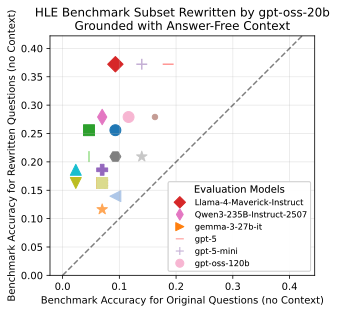
\includegraphics[width=0.8\columnwidth]{figs/gpt20b-afc_hle.pdf}
	\vspace{-0.5em}
	\caption{Rewriting questions 
		%using \texttt{gpt-oss-20b} 
		using answer-free grounding context yields significant accuracy improvement over the original questions as evaluated on a subset of Humanity's Last Exam (HLE). Our intuition is that this approach is similar to asking a student to restate the question before answering it.
		%Questions rewritten by gpt-oss-20b using answer-free grounding context information demonstrate significant benchmark accuracy improvement over the original questions as evaluated on a subset of Humanity's Last Exam (HLE) where validated context information is available. 
	}
	\label{fig:hle-uplift}
	%	\vspace{-1em}   
\end{figure}
LM users often implicitly assume the LM shares their mental model, including their background knowledge, context, and intent.
This can cause them to omit critical background and related information when formulating a query, believing it to be self-evident.
% If its internal assumptions diverge from the user's unstated intent, the resulting output—while potentially factually sound—is perceived as incorrect or irrelevant.
The LM, lacking this context, operates on training data patterns and the explicit text of the prompt. %the patterns in its training data and the explicit text of the prompt. 
When faced with an under-specified query, it must make assumptions to generate a response.
If the model's chosen assumptions do not align with the user's unstated intent, the resulting answer (while potentially factually correct under that assumed interpretation) will be perceived by the user as incorrect, or irrelevant.%, or even as a "hallucination".

While LMs undeniably possess considerable general knowledge; they can struggle with domain-specific or proprietary data absent from public training sets. 
In professional and enterprise workflows, system performance depends on Retrieval-Augmented Generation (RAG) to dynamically construct context for the LM based upon user queries~\citep{lewis2020retrieval,NEURIPS2024_db93ccb6}.
However, current RAG evaluation focuses on retrieval ranking~\citep{yang2024crag,NEURIPS2024_27245589} rather than how models utilize retrieved documents; information which might be relevant without explicitly contain the answer.

%LMs undeniably possess considerable general knowledge; but are inherently weaker with domain-specific and proprietary information. 
%%Operating in professional domains with specialized 
%These domains require access to supplemental private, specialized, and often confidential data absent from any public training corpus. 
%Specifically, with AI systems targeting professional workflows, new types of evaluation are required to characterize LM capability grounded in document populations.
%%For enterprise applications with internal corporate knowledge management the generalized information contained within a pre-trained LM can be insufficient. 
%%These domains require access to private, specialized, and often confidential data absent from any public training corpus. 
%Current approaches involve retrieval systems which dynamically construct context for the LM based upon user queries~\citep{NEURIPS2024_db93ccb6}.
%Contemporary evaluation of Retrieval-Augmented Generation (RAG) systems focuses on ranking quality and retrieval performance~\citep{yang2024crag,NEURIPS2024_27245589} with less emphasis on how to best utilize the retrieved information.
%LM+RAG evaluation is accurate if RAG surfaces the correct answer, but if only relevant information sans answer is retrieved, performance suffers. 

In this work, we explore the impact on system performance of Answer-Free Context (\texttt{AFC})---background information that is relevant to the question but which does not contain the actual answer.
%Our methodology explores how retrieved information impacts LM+RAG system performance; both when the correct answer is surfaced and when only related background information is found.
%document grounded (i.e. LM+RAG) system performance when either the correct answer is surfaced or when only related background information is found. %, as well as when only background relevant information is surfaced.
%Additionally, we demonstrate benchmark accuracy improvement using a contextually grounded question disambiguation rewrite as shown in \Cref{fig:figure1}.
We demonstrate that even when RAG fails to surface a direct answer, the retrieved background information can be used to perform a contextually grounded disambiguation rewrite (\Cref{fig:figure1}). 
This process improves an underspecified query before it is posed to the answering model.
%Our methodology extracts both additional benchmark accuracy and improved contextual grounding by performing a question disambiguation rewrite. 
%This rewrite operates using Answer-Free Context (\texttt{AFC})---background information that is relevant to the question but which does not contain the actual answer. 
%Given a user question and associated \texttt{AFC}, an LM is used to disambiguate and rewrite the question before its posed to the LM for answering.
An example of an original question, associated \texttt{AFC}, and rewritten question are shown below.

\begin{mdframed}[style=spacedframe]
	%	\small
	%	\scriptsize
	\footnotesize
	\textbf{Original question:} What kind of lasers are crystals of zinc suflde used in?
	
	\noindent\textbf{Answer-free context:} Zinc chloride is often added to lumber as a fire retardant and can be used as a wood preservative. It is also used to make other chemicals. Zinc methyl (Zn(CH3)2) is used in a number of organic syntheses. Zinc sulfide (ZnS) is used in luminescent pigments such as on the hands of clocks, X-ray and television screens, and luminous paints. Crystals of ZnS are used in lasers. Zinc sulfate is a chemical in dyes and pigments. Zinc pyrithione is used in antifouling paints.
	
	\noindent\textbf{Rewritten question:} Which portion of the electromagnetic spectrum do lasers that incorporate zinc sulfide (ZnS) crystals generally operate in?
	
	\noindent\textit{(Prompts are given in the Appendix.)}
\end{mdframed}

% Our methodology for extracting both additional benchmark accuracy and improved contextual grounding via question disambiguation rewrites that make use of Answer-Free Context (\texttt{AFC})---background information that is relevant to the question but which does not contain the answer. 
As shown in \Cref{fig:hle-uplift}, this method can improve \texttt{gpt-5-mini} accuracy on a subset of Humanity's Last Exam (HLE) from 0.14 to 0.37. %0.14 on the original questions to 0.37 on the rewritten questions.
%\Cref{fig:hle-uplift} demonstrates the improvement this method provides on a subset of Humanity's Last Exam with validated grounding context, showing \texttt{gpt-5-mini} improving from an accuracy of 0.14 on the original questions to 0.37 on the rewritten questions.


\noindent This work makes the following contributions:
\begin{packed_enum}
%	\item We explore the impact on LM system accuracy of the RAG surfacing the correct answer vs only background information;
%	\item We demonstrate that leveraging \texttt{AFC} for question rewriting can improve model performance; and %answer-free background context for question disambiguation to improve model accuracy; and
%%	\item We compare and contrast simply prepending surfaced dynamic context against using that information for question disambiguation, demonstrating that question rewriting out-performs context prepending.
%%	\item We show that using surfaced context for question disambiguation and rewriting out-performs prepending that information before the question.
%\item We show that this performance uplift requires a distinct rewriting phase and cannot be recovered by simply prepending context to the query.%, suggesting that reducing prompt ambiguity is a unique and necessary step for maximizing LLM utility.
\item Analyzes the performance differential in RAG systems when retrieving direct answers versus purely auxiliary background information; 
\item Introduces a method for leveraging Answer-Free Context (\texttt{AFC}) to disambiguate queries, yielding significant accuracy gains; and 
\item Demonstrates that this accuracy uplift necessitates a distinct rewriting phase, as it cannot be replicated by simply prepending the retrieved context to a prompt. 
\end{packed_enum}




\section{Related Works}

% (maybe) talk in related works about the disconnect between HLE type benchmarks where the model just has to answer, and when tool use (i.e. internet) is available. In modern RAG finding and surfacing relevant and on topic informatino about the question can provide significant alpha. But that requires shifrting the evaluation target from a Model (+tools) to the Model+RAG dynamic context engine system. That second more complex system with grounding documents is much harder to evaluate than an LM in isolation. 


While LMs store significant parametric knowledge, their responses are not grounded in reliable external information sources. %without additional components their responses are not grounded in reliable external information source.
Dynamic context construction approaches like RAG address this by fetching external evidence during the generation process \citep{sharma2025retrieval}.
Grounding the LM response in external (non-parametric) data significantly improves factual accuracy \citep{sharma2025retrieval}.
The RAG pipeline introduces its own optimization challenges, spanning document chunking, search, ranking \citep{NEURIPS2024_db93ccb6}, and post-retrieval processing \citep{dai2025evinote}.
A particularly critical component, with a long history in information retrieval, is the transformation, expansion, and normalization of the users query \citep{Rastogi2019,rivas2014study}.

The initial user query is often an imperfect expression of the underlying information need, suffering from ambiguity, missing context, or terminology poorly aligned with the target document corpus. 
To bridge this lexical gap, modern RAG systems, like their classic predecessors, can employ query expansion and rewriting \citep{jagerman2023query,zhou2023unified,li2024dmqr}.
Query expansion reformulates the question to better surface relevant documents and improve the signal-to-noise ratio of the retrieved context~\citep{gao2023retrieval}.
%The goal is to reformulate the query to better surface relevant documents and improve the signal-to-noise ratio of the retrieved context.

LMs have proven adept at this rewriting, expansion, and contextualization task; disambiguating queries using carefully designed prompts \citep{wilson2025contextualizing,gao2023retrieval,sun2025picos}. 
Other approaches explore post RAG retrieval optimizations for improving signal to noise in the surfaced documents, shifting from a retrieve-generate paradigm to retrieve-note-generate where the discovered documents are summarized into high level notes \citep{dai2025evinote}.

Other dynamic context strategies focus on getting the most out of the documents placed within the LM context.
For example, Step-Back Prompting attempts to have LMs derive high-level concepts from first principles to guide reasoning in query answering \citep{zheng2023take}.
Frameworks like AGREE have the LM cite its sources within the context window (drawn from grounding documents) \citep{ye2023effective}.
Other approaches involve extensions to chain-of-thought including Meta-CoT which models how to determine what underlying reasoning is required to arrive at a particular CoT \citep{xiang2025towards}.
CoT type reasoning approaches enable the LM to employ some form of self-directed question rewriting during the process of figuring out how best to respond.

%While benchmarks exists for end-to-end LM systems with RAG \citep{NEURIPS2024_27245589,yang2024crag}, they can suffer from the same static benchmarking flaws LM knowledge evaluations have. 
%A primary cause of benchmark utility decay is the public and static nature of the test data. 
%Shifting to dynamic generative benchmarking constructed on-demand from trusted document corpora is one solution.
%This approach, exemplified by \citep{majurski2025generative,shashidhar2025yourbench,li2025autobencherdeclarativebenchmarkconstruction}, extends the evaluation landscape by making it possible to create private, domain-specific, and temporally relevant assessments that are inherently resistant to contamination.
%
%%This paradigm empowers users to move beyond generic, one-size-fits-all benchmarks and create evaluations tailored to their specific needs; enabling  more accurate assessment of a model's utility for specific applications.
%%For example, a law firm can generate a benchmark from its case files, a pharmaceutical company can test a model's knowledge of its latest research papers, and a software company can evaluate a model's ability to understand its proprietary codebase. 
%A central tenet of this generative evaluation approach is benchmarks must be grounded in the provided source documents. 
%This means that each question should be verifiably answerable using only the information contained in the source text. 
%This grounding is critical because it shifts the object of evaluation from "what the model knows" (parametric knowledge) to "how the model reasons" over a given context. 
%%Combined with varying levels of compute budget, benchmark-free methods like TreeEval~\citep{li2025treeeval} might serve dynamic context construction LM evaluation well, enabling an adaptive powerful "examiner" LM tasked with probing the target model for weaknesses given a topic. 
%%TreeEval starts by generating initial questions, then dynamically generating follow up based on the initial response building a tree of inquiry, potentially using information sources the model under evaluation does not have access to, enhancing the evaluation asymmetry. 
%%Combining generative benchmarking with document grounding evaluation critically important for next-gen LM system evaluation approaches. 





\section{Methods}

This work explores applying RAG query rewrite/expansion techniques directly to questions posed to LMs, producing an accuracy uplift on evaluation benchmarks. %on direct factual questions posed to LMs.
Benchmarks like MMLU-pro evaluate knowledge by posing factual questions~\citep{wang2024mmlu}.
%To highlight the core problem, \Cref{fig:impact-of-context} shows the impact of context on \texttt{gpt-oss-120b}'s performance (across all datasets used in this study). 
\Cref{fig:impact-of-context} shows the impact of context on \texttt{gpt-oss-120b}'s performance (across all datasets used in this study). 
Queries without any supporting context produce mixed results (blue); \texttt{Question+Context}, in which the prepended context contains the desired answer, performs well (red); and \texttt{Question+AFC} does not match the context-supported accuracy (green).
\begin{figure}[t!]
	\vspace*{-0.25em}
	\centering
	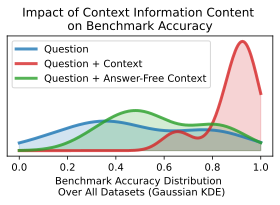
\includegraphics[width=0.75\columnwidth]{figs/impact_of_context_gpt-oss-120b.pdf}
	\vspace{-0.8em}
	{\small
		\caption{The quality of context information presented to the question answering LM has a drastic impact on system performance. Accuracy is high when RAG systems correctly surface context with the answer (red), but when the question is presented without context (blue) or the surfaced information does not contain the answer (green), benchmark performance suffers.}
		\label{fig:impact-of-context}
	}	
	\vspace{-1.0em}   
	
\end{figure}
However, as shown in \Cref{fig:hle-uplift}, using \texttt{AFC} to rewrite the question can both disambiguate what is being asked and fill in relevant background assumptions, producing robust accuracy gains. 
This increase in performance does not rely on model weight knowledge (\texttt{gpt-oss-20b} is an adequate re-writer).
Additionally, just prepending the \texttt{AFC} text before the question does not produce an equivalent accuracy uplift as shown in \Cref{fig:impact-of-rewrite}, where \texttt{Question+Answer-Free Context} under-performs \texttt{Rewritten Question}.
The accuracy uplift effect is caused by the act of interpretation during rewriting, via clarifying and disambiguating the question separately from attempting to answer it. 
\begin{figure}[t!]
	\vspace*{-0.25em}
	\centering
	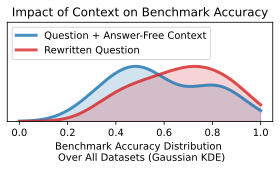
\includegraphics[width=0.75\columnwidth]{figs/qAFC_vs_RQ_gpt120b.pdf}
	\vspace{-0.8em}
	{\small
		\caption{The act of interpretation during question rewriting produces an accuracy uplift beyond just prepending the \texttt{Answer-Free Context} information used to rewrite before the question.}
		\label{fig:impact-of-rewrite}
	}
	\vspace{-1.0em}   
\end{figure}
Its worth noting that question rewriting using \texttt{AFC} does not recover the full performance improvement of surfacing and prepending the grounding context which directly contains the correct answer.

Prior work on RAG systems has demonstrated the utility of query expansion~\citep{wilson2025contextualizing} and prior work on generative benchmarking demonstrated a correlation between generated question length and model benchmark accuracy~\citep{majurski2025generative}.
These two pieces of evidence indicate that applying rewriting to knowledge benchmarks would produce an uplift in accuracy, potentially by placing the LM under evaluation in the right "state of mind" to answer the question better.
This work explores that trend and characterizes how well that effect generalizes, and provides some thoughts on why it might happen. 



\subsection{Datasets \& Models}

To explore the impact of question rewriting on LM benchmark performance, dataset are required which contain pairs of questions with associated context which provides the correct answer.
While most RAG systems are designed to produce that type of information, validated reference data is in short supply. 
Additionally, datasets from post model knowledge cutoff enables evaluating whether the observed effect stems from memorization/recall within the model weights, or whether the question disambiguation approach generalizes to new unseen knowledge. 

\Cref{tab:dataset_publication_cutoff} indicates which datasets were used in this study, and highlights the release data of the benchmark. 
Only Humanity's Last Exam (HLE)~\citep{HumanityLastExam} and the generative benchmarking data was new enough to be post knowledge cutoff for all models tested.

\begin{table}[h!]
	\centering
	\caption{Evaluation Datasets and Publication Dates}
	%	\footnotesize
	\scriptsize
	\label{tab:dataset_publication_cutoff}
	\vspace{-1em}   
	
	\begin{tabular}{p{5.5cm} p{1.25cm}}
		\toprule
		\textbf{Dataset} & \textbf{Release Date}  \\
		Public Datasets & \\
		\toprule
		Humanity's Last Exam~\citep{HumanityLastExam} & Jan 2025\\
		\hline
		Squadv2~\citep{DBLP:journals/corr/abs-1806-03822} & 2018 \\
		\hline
		HotpotQA~\citep{yang2018hotpotqa} & 2018 \\
		\hline
		TrivaQA-web~\citep{2017arXivtriviaqa} & 2017 \\
		\hline
		NaturalQuestionsShort~\citep{kwiatkowski2019natural} & 2019 \\
		\hline
		PubMedQA~\citep{jin2019pubmedqa} & 2019 \\
		\hline
		BoolQ~\citep{clark2019boolq} & 2019 \\
		\hline
		FermiQA~\citep{kalyan2021much} & 2021 \\
		\hline
		MS-MARCO-QA~\citep{bajaj2016ms} & 2016 \\
		\hline
		MusiqueQA~\citep{trivedi2022musique} & 2022 \\
		\hline
		2WikiMultiHopQA~\citep{ho2020constructing} & 2020 \\
		\bottomrule
		\vspace{0.1em}   
		Generative Benchmarks (constructed using~\citep{majurski2025generative}) & \\
		\toprule
		arXiv\_2502\_17521v1~\citep{chen2025recent} & 2025 \\
		\hline
		America's AI Action Plan~\citep{AiPlan} & 2025 \\
		\bottomrule
		\vspace{0.1em}   
		Generative Benchmarks (constructed using~\citep{shashidhar2025yourbench}) & \\
		\toprule
		arXiv\_2502\_17521v1~\citep{chen2025recent} & 2025 \\
		\hline
		America's AI Action Plan~\citep{AiPlan} & 2025 \\
		\bottomrule
	\end{tabular}
	\vspace{-1em} 
\end{table}

% HLE data sourceing https://www.futurehouse.org/research-announcements/hle-exam
% Audited HLE dataset https://huggingface.co/datasets/futurehouse/hle-gold-bio-chem
The originally published HLE dataset does not contains associated context with each question.
However, FutureHouse released manual validation for a subset of chemistry/biology questions with grounding literature~\citep{HleFutureHouse}.
This work used that validated subset of the HLE questions FutureHouse annotated as correctly answered and which had sufficient grounding information.

Evaluating the efficacy of query rewriting for LM benchmark evaluation requires two categories of models. 
First the model doing the question rewriting, note this is not the same as the model under evaluation on the benchmark.
We separate the question rewriting and the evaluation phases to ensure that all evaluation models are given the same rewritten questions to reduce measurement noise. 
Second are the set of models we evaluated using the rewritten questions; these span a wide range of size and capability.
\Cref{tab:model_cutoff} outlines the models we evaluated the rewritten question benchmarks against. 


\begin{table}[h!]
	\centering
	\caption{Evaluation Models Knowledge Cutoff}
	\label{tab:model_cutoff}
	\scriptsize
	\vspace{-1em} 
	
	\begin{tabular}{p{3.6cm} p{1.2cm} p{1.2cm}}
		\toprule
		\textbf{Model} & \textbf{Knowledge-Cutoff} & \textbf{Public-Release}  \\
		\hline
		\texttt{gpt-5} & Sep 2024 & Aug 2025  \\
		\hline
		\texttt{gpt-5-mini} & May 2024 & Aug 2025  \\
		\hline
		\texttt{gpt-5-nano} & May 2024 & Aug 2025  \\
		\hline
		\textbf{\texttt{gpt-oss-20b}} & Jun 2024 & Aug 2025  \\
		\hline
		\textbf{\texttt{gpt-oss-120b}} & Jun 2024 & Aug 2025 \\
		\hline
		\texttt{gemma-3-1b-it} & Aug 2024 & Mar 2025 \\
		\hline
		\texttt{gemma-3-4b-it} & Aug 2024 & Mar 2025 \\
		\hline
		\texttt{gemma-3-12b-it} & Aug 2024 & Mar 2025 \\
		\hline
		\texttt{gemma-3-27b-it} & Aug 2024 & Mar 2025  \\
		\hline
		\texttt{Llama-3.2-3B-Instruct} & Dec 2023 & Sep 2024 \\
		\hline
		\texttt{Llama-3.1-8B-Instruct} & Dec 2023 & Jul 2024 \\
		\hline
		\texttt{Llama-3.3-70B-Instruct} & Dec 2023 & Dec 2024 \\
		\hline
		\texttt{Llama-4-Maverick-Instruct-FP8} &  Aug 2024 & Apr 2025  \\
		\hline
		\texttt{phi-4} & June 2024 & Dec 2024\\
		\hline
		\texttt{Qwen3-1.7B} &  & Apr 2025 \\
		\hline
		\texttt{Qwen3-4B-Instruct-2507} &  & Aug 2025 \\
		\hline
		\texttt{Qwen2.5-7B-Instruct} &  & Sep 2024  \\  
		\hline
		\texttt{Qwen3-30B-A3B-Instruct-2507} &  & Jul 2025 \\
		\hline
		\textbf{\texttt{Qwen3-235B-A22B-Instruct-2507}} &  & Jul 2025  \\
		\bottomrule
	\end{tabular}
	%\vspace{-1em} 
\end{table}


\subsection{Question rewrite procedure}

The question rewriting and expansion was approached as a pre-processing step before benchmarking the evaluation models against the modified questions. 
We evaluated three different LMs for question rewriting: small \texttt{gpt-oss-20b}, medium \texttt{gpt-oss-120b}, and large \texttt{Qwen3-235B-A22B-Instruct-2507}.
These are indicated in \Cref{tab:model_cutoff} with bold.
For each question in each dataset the rewriting LM was provided the original question, correct answer, and grounding context during prompting (\Cref{apx:rewrite-prompt}) to rewrite the question to disambiguate what was being asked.
In addition to rewriting the question the rewriting model must generate what it thinks the correct answer should be, this serves as a validation check against topic drift.
This results in three rewritten variants of each question, one for each of the rewriting models being tested for their ability to successfully perform the rewrite (bold models in \Cref{tab:model_cutoff}).

We filter the rewritten questions to ensure that no degenerate questions are included in the final benchmark.
An LM-Judge is used to extract the following properties: reformatted question similarity to the original question, reformatted answer similarity to the original answer, reformatted question giveaway score, original question giveaway score.
The reformatted question and answer similarity scores are used to discard any questions which are too dissimilar to the original.
The giveaway scores are used to remove any reformatted questions which got easier in the process of rewriting. 
I.e. if the reformatted giveaway score is higher than the original question (the answer is given away more in the rewritten question), that entry is discarded.
This produces a new benchmark for each of the rewriting models that should be strictly more difficult than the original, but with disambiguated questions.



\subsection{Evaluation methodology}

%To evaluate the benchmark accuracy uplift provided by question rewriting and expansion 
Evaluating the efficacy of query rewriting grounded in context requires benchmarking each model under evaluation for three configurations:
{\renewcommand\labelenumi{(\theenumi)}
	\begin{enumerate*} %packed_enum   enumerate
		\item Original Question: the normal benchmarking use case, 
		\item Original Question with Context Prepended: the RAG retrieval use case, and 
		\item Rewriten Question: the uplift imparted by rewriting.
	\end{enumerate*}
}

To quantify the accuracy uplift, we compute the following average per-model and per-dataset differences.
{\renewcommand\labelenumi{(\theenumi)}
	\begin{enumerate*} 
		\item Rewriten Question - Original Question: the direct rewrite uplift, 
		\item Rewriten Question - Original Question with Context Prepended: the rewrite uplift compared to the RAG retrieval use case
	\end{enumerate*}
}
This comparison between the rewritten question and the original question with the context prepended enables evaluating whether the rewrite outperforms benchmarking models with a RAG database which contains only background information.
However, if the context contains the answer, one would expect any benchmarking with the context included to yield roughly 100\% accuracy.
To mitigate this we developed a version of each grounding context that is "Answer-Free". 
\texttt{AFC} was developed using a single LM (\texttt{gpt-oss-120b}) to rewrite the context (see \Cref{apx:afc} for the prompt).
The results section covers the accuracy uplift using the original context (the less interesting use case) as well as the Answer-Free Context (\texttt{AFC}).
\texttt{AFC} replicates the use case where a RAG system surfaces background information, but not the actual answer to the users question. 
Our results demonstrate accuracy uplift in benchmark performance when question rewriting is performed using this Answer-Free Context. 
This uplift effect is larger than just prepending the \texttt{AFC}.

To characterize one hypothesis for why this affect shows up, we leverage an embedding model (\texttt{e5-mistral-7b-instruct}) to understand the change in cosine distance between the original question and the context compared to the cosine distance between the rewritten question and the context.
We demonstrate that improvements in benchmark accuracy correlate with reductions in the cosine distance between the question and context.
In other words, the rewritten question appears to place the model closer to the right frame of mind to answer the question, as the cosine distance between the question and the context is smaller after the rewrite.

% TODO continue editing

\section{Results}
% gpt-5-mini on HLE rewrite using gpt-oss-20b
% orig = 0.139
% rewrite = 0.372
\Cref{fig:figure1} outlines the accuracy uplift for all evaluated models on just the HLE-subset dataset.
Given that \texttt{gpt-oss-20b} leveraged Answer-Free Context for question rewriting, the accuracy improvement in models like \texttt{gpt-5-mini} (from 13.9\% to ~37.2\%) is remarkable.
To validate that our Answer-Free Context is not in fact giving away the answer, we plot the performance of all models across all datasets comparing the original question accuracy to the benchmark accuracy with the context prepended before the question during benchmark evaluation. 
\begin{figure}[h!]
	\vspace*{-0.5em}
	\centering
	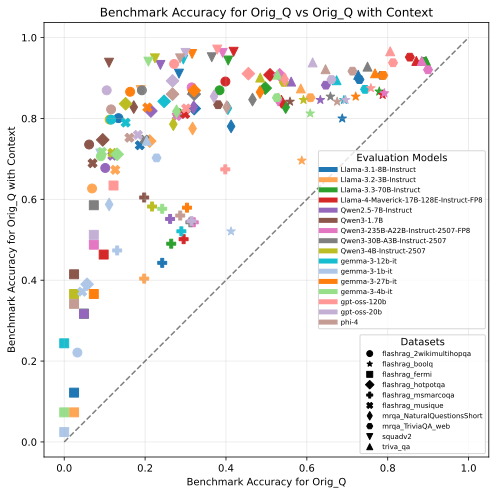
\includegraphics[width=0.9\columnwidth]{figs/data-subset-500-gpt120b-orig-giveaway.pdf}
	\vspace{-0.8em}
	\caption{Scatterplot of benchmark accuracy values per-dataset and per-model plotting the original question accuracy against the original question prepended with the answer-containing context, resulting in significant over-performance.}
	\label{fig:orig-giveaway}
	%	\vspace{-1em}   
\end{figure}
\Cref{fig:orig-giveaway} scatterplots the original question benchmark accuracy on the x-axis vs the original question with associated context on the y-axis.
For most models and datasets prepending the answer-containing context provides significant uplift in benchmark accuracy.
In comparison, \Cref{fig:orig-giveaway-afc} scatterplots the same values but prepending the Answer-Free Context instead.
\begin{figure}[h!]
	%	\vspace{-1.0em}
	\centering
	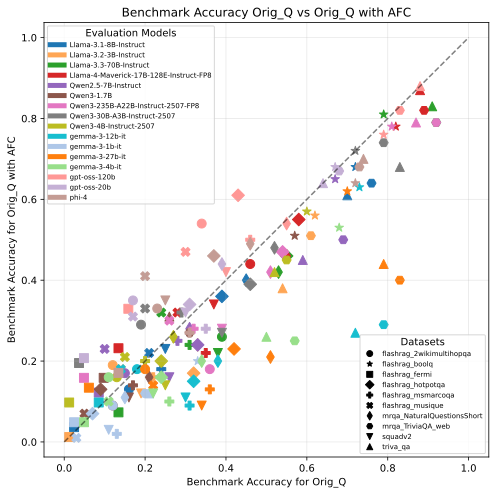
\includegraphics[width=0.9\columnwidth]{figs/data-subset-500-afc-gpt120b-orig-giveaway.pdf}
	\vspace{-0.8em}
	\caption{Scatterplot of benchmark accuracy values per-dataset and per-model plotting the original question accuracy against the original question prepended with the answer-free context, resulting in no trend of accuracy improvement attributable to the context.}
	\label{fig:orig-giveaway-afc}
	%	\vspace{-1em}   
\end{figure}
This results in no pattern of accuracy uplift attributable to the AFC, indicating the the answer removal process was successful.


To compare the per-dataset per-model benchmark accuracy uplift, \Cref{fig:r_minus_q} plots the distribution in accuracy improvement measured as the rewritten question accuracy minus the original question accuracy. 
This demonstrates that models benchmark better on the rewritten question compared to the original questions, but considering the rewritten questions likely contain more detailed information drawn from context, its not a fair comparison. 
\begin{figure}[h!]
	\vspace{-0.5em}
	\centering
	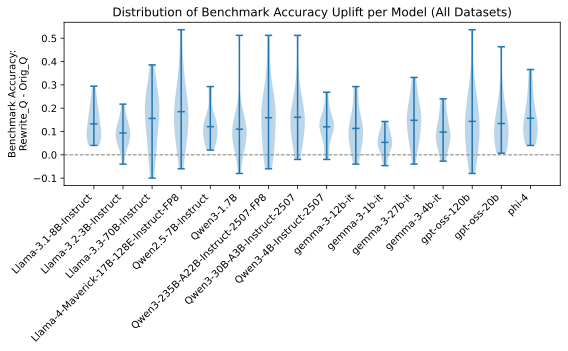
\includegraphics[width=0.9\columnwidth]{figs/acc_uplift_gpt120/r_minus_q.pdf}
	\vspace{-0.8em}
	\caption{Per-dataset per-model difference in benchmark accuracy between the rewritten question and the original question. The violin plot distribution highlights the range of accuracy deltas over all datasets for each model evaluated.}
	\label{fig:r_minus_q}
	\vspace{-1em}   
\end{figure}
\FloatBarrier
To demonstrate the accuracy uplift from rewriting under the worst possible conditions, \Cref{fig:r_minus_q_afc_giveaway} plots the accuracy of the rewritten questions minus the original questions with the answer-free context prepended. 
Note, the question rewriting process only used the answer-free context, so both the rewritten question and the original question with AFC are on even footing information-wise.
%Additionally, the model under evaluation has access to all of the information the rewriting model did, but the task is question answering instead of disambiguation, resulting in lower benchmark accuracy compared to a separate rewrite then answer paradigm.
Additionally, the model under evaluation has access to all information the rewriting model did. 
This demonstrates that the act of rewriting the questions in a separate rewrite-then-answer paradigm produces an accuracy improvement that is not possible by just prepending the same information into the models context during evaluation.
\begin{figure}[h!]
	\vspace{-0.5em}
	\centering
	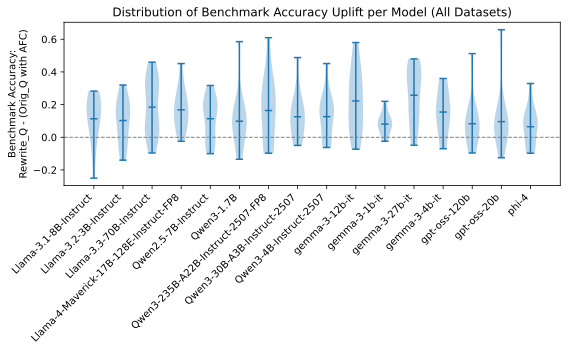
\includegraphics[width=0.9\columnwidth]{figs/acc_uplift_gpt120/rafc_minus_qafc_giveaway.pdf}
	\vspace{-0.8em}
	\caption{Violin plots of the per-dataset per-model difference in benchmark accuracy between the rewritten questions and the original questions with associated answer-free context. The violin plot distribution highlights the range of accuracy deltas over all datasets for each model evaluated.}
	\label{fig:r_minus_q_afc_giveaway}
	\vspace{-1em}   
\end{figure}

The violin plot information can be visualized using a scatterplot to break out the effects of model and dataset; where the x-axis is the original benchmark accuracy and the y-axis is the rewritten question performance. 
\Cref{fig:gpt120b-afc} showcases the results from all datasets before model knowledge cutoffs. 
All dataset and model combinations lie above the $y=x$ line which indicates identical performance between the original and rewritten questions. 
Some dataset model combinations get more uplift than others, but there are no combinations where benchmark performance decreases. 
\begin{figure}[h!]
	\vspace{-0.5em}
	\centering
	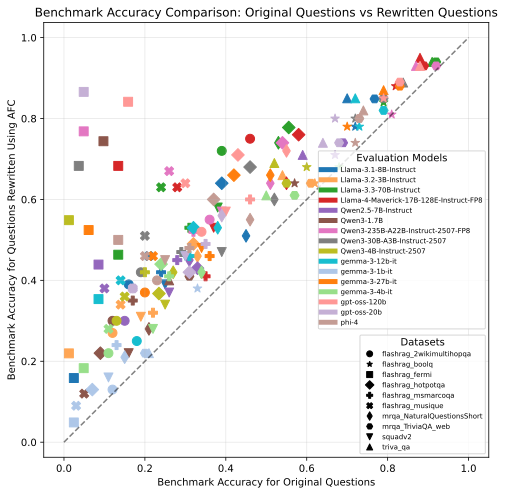
\includegraphics[width=0.9\columnwidth]{figs/gpt120b-afc.pdf}
	\vspace{-0.8em}
	\caption{Scatterplot showing the per-dataset per-model improvement in benchmark accuracy caused by rewriting the question. The x-axis shows the original question benchmark accuracy while the y-axis shows the rewritten question benchmark accuracy.}
	\label{fig:gpt120b-afc}
	%	\vspace{-1em}   
\end{figure}
Additionally, some datasets like \texttt{flashrag\_fermi} demonstrate significant uplift stemming from disambiguation. 

Breaking out the benchmark accuracy uplift results per-dataset reveals an interesting exception, comparing the rewritten HLE-subset to the original questions with the answer-free context prepended demonstrates the only consistent drop in accuracy, as shown in \Cref{fig:r_minus_q_afc_giveaway_dataset}.
In \Cref{fig:r_minus_q_afc_giveaway_dataset} the first 5 datasets are from post knowledge cutoff, and the remainder before. 
Additionally, due to a paucity of datasets released since the beginning of the year, all but the HLE-subset were generativly created benchmarks using wither \citep{majurski2025generative} or \citep{shashidhar2025yourbench}.
Those benchmarks tend to have more complex questions that are less fact based than the extractive QA datasets which make up the majority. 
Thus, they demonstrate minimal benchmark accuracy uplift from rewriting compared to just prepending the answer-free context.
This trend extends to the HLE-subset which has the most complex and difficult questions over all the datasets.
Therefore, there is a trend that fact based benchmarking is improved by the question rewrite, whereas questions where you need to reason through and think about the question don't.
These trends are demonstrated in \Cref{fig:figure1} the rewritten HLE questions provide significant accuracy uplift compared to the original questions, but less than just prepending the answer-free context.
\begin{figure}[h!]
	\vspace{-0.5em}
	\centering
	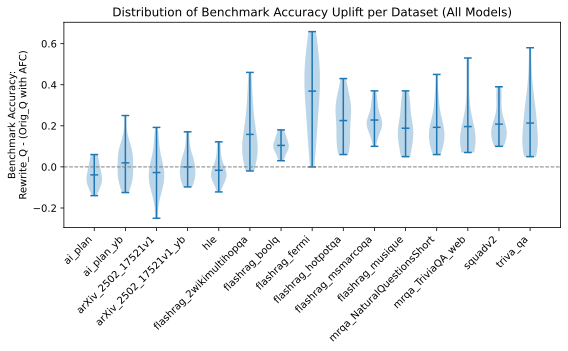
\includegraphics[width=0.9\columnwidth]{figs/acc_uplift_gpt120/rafc_minus_qafc_giveaway_dataset.pdf}
	\vspace{-0.8em}
	\caption{Violin plots of the per-dataset per-model difference in benchmark accuracy between the rewritten questions and the original questions with associated answer-free context. The violin plot distribution highlights the range of accuracy deltas over all models for each dataset evaluated.}
	\label{fig:r_minus_q_afc_giveaway_dataset}
	\vspace{-1em}   
\end{figure}

Our hypothesis is that the benchmark accuracy improvement from reformatting the questions with answer-free context stems from disambiguation and improving the concept alignment between the question and the underlying context information.
To demonstrate this we plot the improvement in benchmark accuracy between the rewritten question and original question against the improvement in cosine similarity between the question and context when questions are rewritten.
\Cref{fig:acc_vs_embedding_gpt120b_e5-mistral-7b-instruct} demonstrates that most scattterplot points end up in the upper right quadrant, where improvements in benchmark accuracy correlate with improvements in cosine similarity between the question and context.
In other words, rewritten questions that have a higher cosine similarities to the context also have a higher benchmark accuracy.
Its worth noting that for every model and dataset combination pre-knowledge cutoff these points all landed in the upper right quadrant.
However, for some models in the post-knowledge cutoff datasets there is a drop in benchmark accuracy as evidenced by those points in the upper left quadrant. 
Each dataset has a distribution of accuracy improvements across the evaluated models, which is why the datasets in \Cref{fig:acc_vs_embedding_gpt120b_e5-mistral-7b-instruct} forms horizontal bands.
\begin{figure}[h!]
	\vspace{-0.5em}
	\centering
	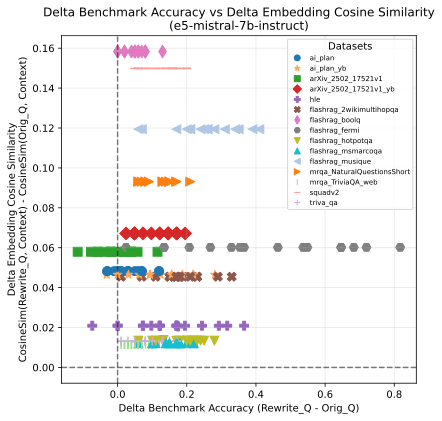
\includegraphics[width=0.9\columnwidth]{figs/acc_vs_embedding_gpt120b_e5-mistral-7b-instruct.pdf}
	\vspace{-0.8em}
	\caption{Scatterplot plotting the benchmark accuracy improvement on the x-axis vs improvement in cosine similarity between the question and context for rewritten questions on the y-axis. The x-axis plots delta benchmark accuracy Rewrite\_Q - Orig\_Q. Larger values indicate the rewritten question improved benchmark accuracy. The y-axis plots the increase in cosine similarity between the question and context resulting from rewriting. Larger values indicate better alignment between Rewrite\_Q and AFC compared to Orig\_Q and AFC. That all points are in the upper right quadrant indicates that improvements in embedding alignment between the question and grounding context correlates with improvements benchmark accuracy.}
	\label{fig:acc_vs_embedding_gpt120b_e5-mistral-7b-instruct}
	%	\vspace{-1em}   
\end{figure}


If question rewriting has a positive impact on benchmark accuracy above and beyond using the answer-free context to ground the response, could that be incorporated into the CoT prompting?
\Cref{fig:insitu_rafc_minus_q_afc_giveaway_dataset} demonstrates that attempting to move this rewrite operations into benchmark evaluation as a single operation does not produce the accuracy uplift. 
This holds both for models with \texttt{<thinking>} support and those without. 
This was evaluated by using the same question rewriting prompt lightly modified to tell the LM under evaluation to first rewrite the question for disambiguation before answering the rewritten question using the same formatting as all other LM benchmarking used in this study. 
\Cref{fig:insitu_rafc_minus_q_afc_giveaway_dataset} compares the Insitu\_Rewrite\_Q to the Orig\_Q with AFC, so the same information is presented to both evaluation runs, the only difference is in the prompting directions to first rewrite instead of just directly answer. 
\begin{figure}[h!]
	\vspace{-0.5em}
	\centering
	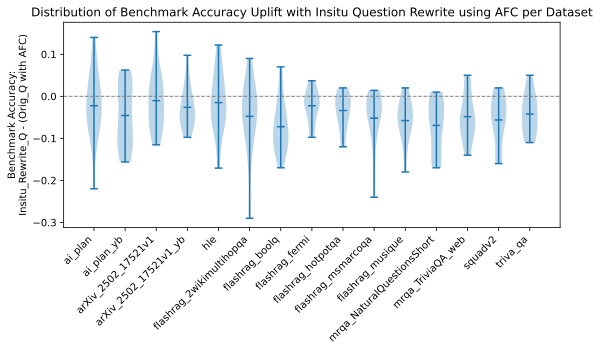
\includegraphics[width=0.9\columnwidth]{figs/insitu_rafc_minus_q_afc_giveaway_dataset.pdf}
	\vspace{-0.8em}
	\caption{Per-dataset improvement in benchmark accuracy from performing an insitu-rewrite of the question using answer-free context during benchmark evaluation. This combines the rewrite-then-answer into a single operation. The prior accuracy improvement disappears highlighting the impact of task separation between the rewrite and answer phases.}
	\label{fig:insitu_rafc_minus_q_afc_giveaway_dataset}
	%	\vspace{-1em}   
\end{figure}


\subsection{Limitations}

The evaluation of the impact of question rewriting relies heavily on extractive QA datasets which have paired question and context tuples.
The exception is the HLE-subset where the questions are post-facto grounded using internet search.
Thus many of the fact-based extractive QA dataset questions are easily answerable when the LM is presented the answer-containing context. 
This limitation is primarily a result of the availability of public dataset of questions paired with grounding context.

\section{Conclusion}

When provided grounding context without the correct answer, LM benchmarking accuracy can be improved by following a similar question disambiguation rewriting policy that information retrieval literature has been leveraging.
This question rewriting does not require that the dynamic context system (i.e. RAG) has found and surfaced the answer to the users question, only that is discovered relevant background information. 
Comparing the rewritten question benchmark accuracy to the original question with associated answer-free context prepended reveals strong uplift attributable to the rewriting process, and not just the inclusion of relevant information into the context window. 
Additionally, the separation of tasks into rewrite-then-answer provides accuracy improvements that prompt modification alone cannot (\Cref{fig:insitu_rafc_minus_q_afc_giveaway_dataset}). 
This holds true for models with and without formalized "reasoning" capability. 

A notable exception to this uplift is the comparison between rewritten questions and original questions with AFC for the more complex questions in the generative benchmark dataset and the HLE-subset.
\Cref{fig:r_minus_q_afc_giveaway_dataset} demonstrates that for these highly detailed and complex questions, simply prepending the answer-free context provides equivalent or better performance improvements to attempting to rewrite the questions. 
Considering the answer-free context contains significantly more background information than the rewritten question can possible contain, perhaps it isn't to surprising the rewritten question alone cannot provide the full uplift that AFC context can, especially for competent models which can reason over that context.

Interestingly enough, the rewritten question with AFC usually out-performs the original question with AFC. 
\Cref{fig:rafc_giveaway_minus_qafc_giveaway_dataset} highlights that accuracy uplift, with the Fermi reasoning estimation dataset demonstrating significant uplift. 

\begin{figure}[h!]
	\vspace{-0.5em}
	\centering
	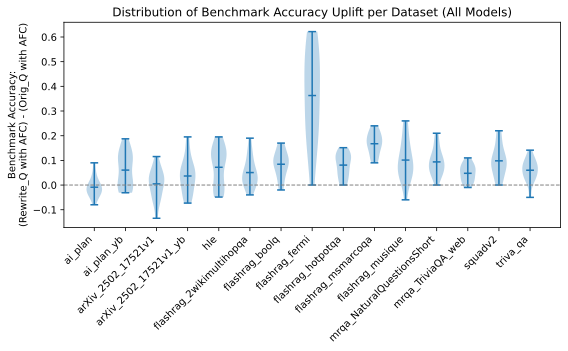
\includegraphics[width=0.9\columnwidth]{figs/acc_uplift_gpt120/rafc_giveaway_minus_qafc_giveaway_dataset.pdf}
	\vspace{-0.8em}
	\caption{Per-dataset improvement in benchmark accuracy from the Rewrite\_Q with AFC compared to the Orig\_Q with AFC during benchmark evaluation. This highlights that both the question rewriting and the addition of the answer-free context improve benchmark accuracy.}
	\label{fig:rafc_giveaway_minus_qafc_giveaway_dataset}
	%	\vspace{-1em}   
\end{figure}





%\subsection{Future work}
%TODO: 
%- characterize the change in question length from orig to rewrite. I.e. how many tokens are being added to disambiguate. 
%- measure the alignment and utility of the context (orig and afc) w.r.t. the question. I.e. does the improvement in answer accuracy correlate with the context utility? i.e. does the reduction in accuracy from orig+giveaway (below the trendline) stem from useless information being included? I.e. would the post-cutoff trend above the trendline return if we only considered those questions where the context paragraph has known utility?



\newpage
\bibliographystyle{plainnat}
{\small
	\bibliography{references}
}

\newpage
\appendix

\section{Impact of Rewrite on Benchmarks}
\label{apx:rewrite_impact}

\Cref{fig:r_minus_q_apx} presents the distribution of accuracy improvement measured as ($\texttt{Rewrite\_Q} - \texttt{Orig\_Q}$) per-evaluation model across all datasets. 
This demonstrates question rewriting broadly improves benchmark accuracy. %the rewritten questions produce broadly improved benchmark performance for all models compared to the original questions.
\begin{figure}[h!]
	\vspace{-0.5em}
	\centering
	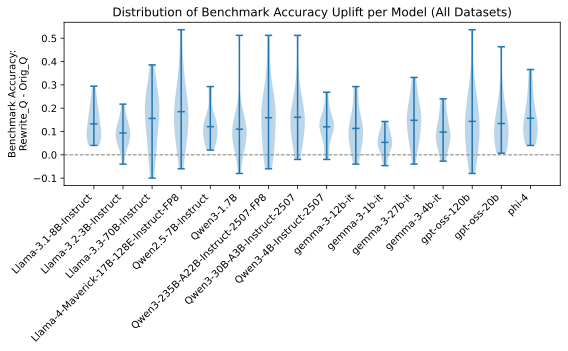
\includegraphics[width=0.9\columnwidth]{figs/acc_uplift_gpt120/r_minus_q.pdf}
	\vspace{-0.8em}
	\caption{Per-dataset per-model difference in benchmark accuracy between the rewritten question and the original question. The violin plot distribution highlights the range of accuracy deltas over all datasets for each model evaluated. Benchmark accuracy improved by an average of 0.1303.}
	\label{fig:r_minus_q_apx}
	% \vspace{-1em}   
\end{figure}
\FloatBarrier

\Cref{fig:r_minus_q_dataset_apx} presents the distribution of accuracy improvement measured as ($\texttt{Rewrite\_Q} - \texttt{Orig\_Q}$) per-dataset instead of per-model like \Cref{fig:r_minus_q_apx}.
\begin{figure}[h!]
	\vspace{-0.5em}
	\centering
	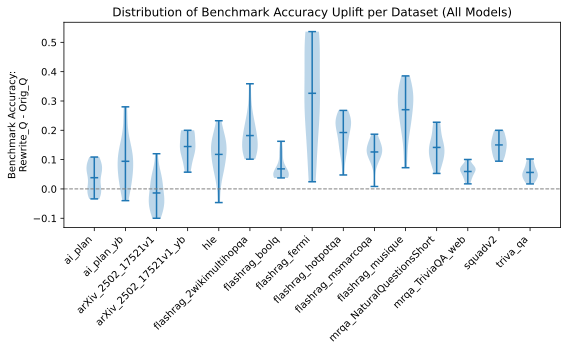
\includegraphics[width=0.9\columnwidth]{figs/acc_uplift_gpt120/r_minus_q_dataset.pdf}
	\vspace{-0.8em}
	\caption{Per-dataset per-model difference in benchmark accuracy between the rewritten question and the original question. The violin plot distribution highlights the range of accuracy deltas over all datasets for each model evaluated. Benchmark accuracy improved by an average of 0.1303.}
	\label{fig:r_minus_q_dataset_apx}
	% \vspace{-1em}   
\end{figure}
\FloatBarrier

%The violin plot information in \Cref{fig:r_minus_q} can be visualized using a scatterplot to break out the effects of model and dataset; where the x-axis is the original benchmark accuracy and the y-axis is the rewritten question performance. 
%\Cref{fig:gpt120b-afc} showcases the results from all datasets before model knowledge cutoffs. 
%All dataset and model combinations lie above the $y=x$ line which indicates identical performance between the original and rewritten questions. 
%Some dataset model combinations get more uplift than others, but there are no combinations where benchmark performance decreases. 

\Cref{fig:r_minus_q_afc_giveaway_apx} presents the distribution of accuracy improvement measured as ($\texttt{Rewrite\_Q} - \texttt{Orig\_Q+AFC}$) per-evaluation model across all datasets. 
\begin{figure}[h!]
	\vspace{-0.5em}
	\centering
	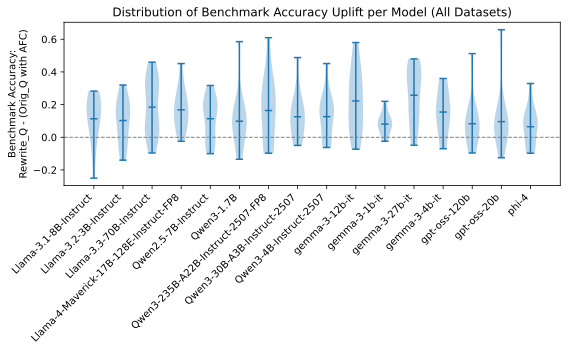
\includegraphics[width=0.9\columnwidth]{figs/acc_uplift_gpt120/rafc_minus_qafc_giveaway.pdf}
	\vspace{-0.8em}
	\caption{Per-model difference in benchmark accuracy between the rewritten questions and the original questions with associated answer-free context. The violin plot distribution highlights the range of accuracy deltas over all datasets for each model evaluated. Benchmark accuracy improved by an average of 0.1346.}
	\label{fig:r_minus_q_afc_giveaway_apx}
	% \vspace{-1em}   
\end{figure}
\FloatBarrier

\Cref{fig:r_minus_q_afc_giveaway_dataset_apx} presents the same information as \Cref{fig:r_minus_q_afc_giveaway_apx}, but with each violin distribution per-dataset instead of per-model.
\begin{figure}[h!]
	\vspace{-0.5em}
	\centering
	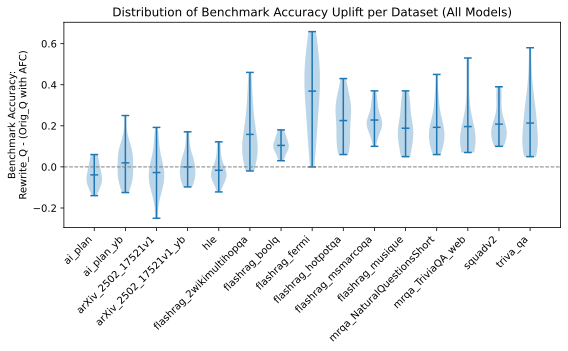
\includegraphics[width=0.9\columnwidth]{figs/acc_uplift_gpt120/rafc_minus_qafc_giveaway_dataset.pdf}
	\vspace{-0.8em}
	\caption{Per-dataset per-model difference in benchmark accuracy between the rewritten questions and the original questions with associated answer-free context. The violin plot distribution highlights the range of accuracy deltas over all models for each dataset evaluated. Benchmark accuracy improved by an average of 0.1346.}
	\label{fig:r_minus_q_afc_giveaway_dataset_apx}
	% \vspace{-1em}   
\end{figure}
\FloatBarrier

\Cref{fig:rafc_giveaway_minus_qafc_giveaway_dataset_apx} demonstrates the benchmark accuracy distribution per-dataset of \texttt{Rewrite\_Q+AFC - Orig\_Q+AFC}.
This combination limits the potential accuracy improvement but reduces the number of datasets which show no average improvement in accuracy.
This may indicate that disambiguation and context inclusion are complementary.
\begin{figure}[h!]
	\vspace{-0.5em}
	\centering
	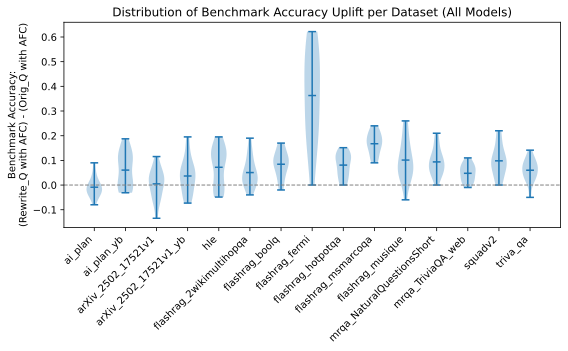
\includegraphics[width=0.9\columnwidth]{figs/acc_uplift_gpt120/rafc_giveaway_minus_qafc_giveaway_dataset.pdf}
	\vspace{-0.8em}
	\caption{Per-dataset improvement in benchmark accuracy from \texttt{Rewrite\_Q} with \texttt{AFC} compared to the \texttt{Orig\_Q} with \texttt{AFC} during benchmark evaluation. Benchmark accuracy improved by an average of 0.0875.}
	\label{fig:rafc_giveaway_minus_qafc_giveaway_dataset_apx}
	%	\vspace{-1em}   
\end{figure}
\FloatBarrier








\section{Question Rewriting Prompt}
\label{apx:rewrite-prompt}

{\scriptsize % \footnotesize
	\begin{lstlisting}[language=json]
		QUESTION_REFORMAT_PROMPT = """
		## Your Role
		
		You are an expert educational content creator specializing in editing and improving evaluation questions to determine the competency of domain experts based on the provided textual information. 
		
		## Input Structure
		
		Your input consists of:
		
		<question>
		[A question to be answered.]
		</question>
		
		<answer>
		[The correct answer to the question.]
		</answer>
		
		<context>
		[The text segment containing information relevant to the question.]
		</context>
		
		## Primary Objective
		
		Your goal is to reformat, rephrase, and rewrite the question according to the provided instructions. The rewritten question should be semantically equivalent to the original question, rewritten for clarity while preserving the same correct answer. This should only be accomplished by filling in background information and explicitly stating assumptions. You are creating a test/quiz question, so DO NOT include the answer information in the question, as that would be a giveaway which skews the results. NEVER include the answer or information which would give away the answer in the rewritten question.
		
		## Analysis Phase
		
		Conduct careful analysis within `<document_analysis>` tags, following these steps:
		
		1. **Thoughtful Content Examination**
		- Carefully analyze the given context, question, and answer; identifying central ideas, nuanced themes, and significant relationships within it.
		
		2. **Concept Exploration**
		- Consider implicit assumptions, subtle details, underlying theories, and potential applications of the provided information.
		
		3. **Intentional Question Planning**
		- Plan how the question can invite deeper understanding, meaningful reflection, or critical engagement, ensuring the question is purposeful.
		
		4. **Detailed Assumption Expansion**
		- Consider what knowledge the question is asking about, and what information and assumptions have been made when formatting the question. Your goal is to provide all the background information and explicitly state assumptions to enhance the clarity of the question.
		
		5. **Giving Away the Answer**
		- Plan how to avoid giving away the answer in the rewritten question. 
		- NEVER include the answer or information which would give away the answer in the rewritten question.
		
		### Documentation in Analysis:
		
		- Clearly document the rationale in the `<document_analysis>` tags, explaining your reasons for exclusion or inclusion decisions.
		- Clearly document what elements of the question need to be disambiguated. What steps need to be taken and what information needs to be include most clearly and concisely disambiguate the question. 
		- Clearly document what information needs to be avoided in the rewritten question to prevent giving away the answer. For example if the question asks about what year a person was born, the question should not include birthday in the biographical details.
		
		
		## Question Rewriting Guidelines
		
		### Encouraged Question Characteristics:
		
		- **Thoughtful Engagement**: Prioritize creating questions that inspire deeper thought and nuanced consideration.
		- **Deep Understanding and Insight**: Ensure that the question and answers require a deep understanding of the content by a professional domain expert.
		- **Self-contained Clarity**: Questions and answers should contain sufficient context, clearly understandable independently of external references.
		- **Brevity**: The rewritten question should be as short as is reasonable while still being clear, understandable, self-contained, and unambiguous.
		
		### Permitted Question Types:
		
		- Analytical
		- Application-based
		- Clarification
		- Counterfactual
		- Understanding
		- Conceptual
		- Factual
		- Open-ended
		- False-premise
		- Edge-case
		- Inference
		- Implication
		- Prediction
		
		(You do not need to use every question type, only those naturally fitting the content and instructions.)
		
		## Output Structure
		
		Present your final output strictly adhering the `<output_format>` tags.
		<output_format>
		Question: [ Question Text ]
		Explanation: [Brief explanation of why the answer is correct]
		Correct Answer: [Short answer]
		</output_format>
		
		## Output
		
		Begin by thoughtfully analyzing the provided context within `<document_analysis>` tags. Then present the resulting formatted question answer pair clearly within `<output_format>` tags.
		
		## Important Notes
		
		- NEVER modify the core element the question is asking about. The knowledge being evaluated shall not change. 
		- Question disambiguation and modification must be grounded in the `<context>`. 
		- Maintain clear, direct, and accurate citations/explanations drawn verbatim from the provided context.
		- Each "thought_process" should reflect careful consideration and reasoning behind your response.
		- When rewriting questions, NEVER include phrases like 'as per the text,' 'according to the document,' or any similar explicit references. Questions should inherently integrate content naturally and stand independently without explicit references to the source material. Make sure that the question is answerable by a domain expert **without the context paragraph**. 
		- Include all relevant context information in the question. Make the question as long and detailed as required so that the test taker can fully understand what is being asked.
		- NEVER include the answer in the rewritten question.
		- Ensure rigorous adherence to output formatting and generate a single `<output_format>` tag block.
		- Verify that the correct answer is in fact correct and the best version of that answer.
		- Verify that the question and answer are semantically equivalent to the original question and answer.
		
		
		
		<question>{question}</question>
		<answer>{answer}</answer>
		<context>{context}</context>
		"""
	\end{lstlisting}
}





\section{Answer-Free Context Creation}
\label{apx:afc}

{\scriptsize % \footnotesize
	\begin{lstlisting}[language=json]
		ANSWER_FREE_CONTEXT_PROMPT = """
		## Your Role
		
		You are an expert educational content creator specializing in editing and improving evaluation questions to determine the competency of domain experts based on the provided textual information. 
		
		## Input Structure
		
		Your input consists of:
		
		<question>
		[A question to be answered.]
		</question>
		
		<answer>
		[The correct answer to the question.]
		</answer>
		
		<context>
		[The text segment containing information relevant to the question.]
		</context>
		
		## Primary Objective
		
		Your goal is to reformat, rephrase, and rewrite the context information according to the provided instructions. The rewritten context should be minimally modified, and semantically equivalent to the original context. The rewrite should only remove the information which gives away the answer to the question. You are creating background material for a test/quiz question, so you need to COMPLETLELY remove the information which gives away the answer to the question from the context. NEVER include the answer or information which would give away the answer in the rewritten context.
		
		## Analysis Phase
		
		Conduct careful analysis within `<document_analysis>` tags, following these steps:
		
		1. **Thoughtful Content Examination**
		- Carefully analyze the given context, question, and answer; identifying central ideas, nuanced themes, and significant relationships within it.
		
		2. **Concept Exploration**
		- Consider implicit assumptions, subtle details, underlying theories, and potential applications of the provided information.
		
		3. **Intentional Context Planning**
		- Plan how the context information can support disambiguation of the question, while not giving away the answer; ensuring the question is purposeful.
		
		4. **Detailed Assumption Expansion**
		- Consider what knowledge the question is asking about, and what information and assumptions have been made when formatting the question. Your goal is to edit the context to remove the information which would give the questions answer away to the test taker.
		
		5. **Giving Away the Answer**
		- Plan how to avoid giving away the answer in the rewritten context. 
		- Figure out what minimal set of information needs to be removed to avoid giving away the answer.
		- NEVER include the answer or information which would give away the answer in the rewritten context.
		
		### Documentation in Analysis:
		
		- Clearly document the rationale in the `<document_analysis>` tags, explaining your reasons for exclusion or inclusion decisions.
		- Clearly document what elements of the context need to be modified. What steps need to be taken and what information needs to be include most clearly and concisely (with minimal modification) remove the answer information from the context. 
		- Clearly document what information needs to be avoided in the rewritten context to prevent giving away the answer. For example if the question asks about what year a person was born, the context should not include birthday in the biographical details.
		
		
		## Context Rewriting Guidelines
		
		## Output Structure
		
		Present your final output strictly adhering the `<output_format>` tags.
		<output_format>
		[ Rewritten Context ]
		</output_format>
		
		## Output
		
		Begin by thoughtfully analyzing the provided question, answer and context within `<document_analysis>` tags. Then present the resulting edited context within `<output_format>` tags.
		
		## Important Notes
		
		- NEVER modify what the question is asking about. NEVER modify the answer. The knowledge being evaluated SHALL NOT change. 
		- Each "thought_process" should reflect careful consideration and reasoning behind your response.
		- NEVER include the answer in the rewritten context.
		- ONLY minimally modify the context as required to remove the answer information. The modified context should be as similar to the original as possible, with the answer information removed. 
		- ONLY remove answer information, do not add new information, and do not remove extraneous information.
		- Ensure rigorous adherence to output formatting and generate a single `<output_format>` tag block.
		
		
		
		<question>{question}</question>
		<answer>{answer}</answer>
		<context>{context}</context>
		"""
	\end{lstlisting}
}



\section{Answer Explanation Validation Prompt}
\label{apx:answer_validation}

{\scriptsize % \footnotesize
	\begin{lstlisting}[language=json]
		EXPLANATION_VALIDATION_PROMPT = """
		## Your Role
		
		You are an expert evaluator of educational content. Your goal is to produce meaningful, insightful knowledge about domain expert evaluations designed to determine competence and knowledge. 
		
		## Input Structure
		
		Your input consists of:
		
		<question>
		[A question to be answered.]
		</question>
		
		<answer>
		[The student's answer to the question.]
		</answer>
		
		<explanation>
		[An explanation for why the answer is correct.]
		</explanation>
		
		<context>
		[The text segment containing information relevant to the question.]
		</context>
		
		## Primary Objective
		
		You will be evaluating and judging the whether the student's answer and their explanation of why their answer is correct makes sense and is logically valid.
		
		Your goal is to judge whether the information presented in `<answer>` is in fact the correct answer to the `<question>` given the information in the `<context>` and whether the `<explanation>` for why the answer is correct is valid. The information in `<context>` and `<question>` can be assumed true, only the context of `<answer>` needs to be validated for correctness.
		
		### Metrics
		
		1. **Answer Correctness:** Rate from 1 to 10 how correct the provided student answer is given the information in the `<question>` and `<context>`. A rating of 1 indicates the answer is incorrect. A rating of 10 indicates the answer is correct and complete. 
		
		2. **Explanation Validity:** Rate from 1 to 10 how valid the students `<explanation>` of their answer is. The `<explanation>` should explain their thinking and the information used to determine the correct answer given the context and question. Low ratings indicate the explanation is not valid, correct, or that there is some flaw in the thinking or logic of the student. High ratings indicate the explanation is valid, correct, and explains why the answer is what it is. 
		
		## Analysis Phase
		
		Conduct careful analysis within `<document_analysis>` tags, following these steps:
		
		1. **Thoughtful Content Examination**
		- Carefully analyze the given context, identifying central ideas, nuanced themes, and significant relationships within it.
		
		2. **Concept Exploration**
		- Consider implicit assumptions, subtle details, underlying theories, and potential applications of the provided information.
		
		## Output Structure
		
		Present your final output strictly adhering the `<output_format>` tags.
		<output_format>
		Answer Correctness: [ Correctness Rating. Respond with a number in [1, 2, 3, 4, 5, 6, 7, 8, 9, 10] ]
		Explanation Validity: [ Validity Rating. Respond with a number in [1, 2, 3, 4, 5, 6, 7, 8, 9, 10] ]
		</output_format>
		
		## Output
		
		Begin by thoughtfully analyzing the provided context within `<document_analysis>` tags. Then present the resulting formatted question answer pair clearly within `<output_format>` tags.
		
		## Important Notes
		
		- Each "thought_process" should reflect careful consideration and reasoning behind your ratings.
		- Ensure rigorous adherence to output formatting.
		
		
		<question>{question}</question>
		<answer>{answer}</answer>
		<explanation>{explanation}</explanation>
		<context>{context}</context>
		"""
	\end{lstlisting}
}



\section{Question Property Validation Prompt}
\label{apx:question_validation}

{\scriptsize % \footnotesize
	\begin{lstlisting}[language=json]
		PROPERTIES_PROMPT = """
		## Your Role
		
		You are an expert evaluator of educational content. Your goal is to produce meaningful, insightful knowledge about domain expert evaluations designed to determine competence and knowledge. 
		
		## Input Structure
		
		Your input consists of:
		
		<question>
		[A question to be answered.]
		</question>
		
		<answer>
		[The correct answer to the question.]
		</answer>
		
		<context>
		[The text segment containing information relevant to the question.]
		</context>
		
		## Primary Objective
		
		You will be evaluating and judging the quality of test and evaluation questions across a variety of metrics. Your goal is to judge and evaluate the quality of various test and evaluation questions across a variety of metrics. The `<question>` and `<answer>` pair is grounded and drawn from the `<context>`. 
		
		### Metrics
		
		1. **Clarity:** Rate from 1 to 10 the clarity and comprehensibility (how understandable it is) of the provided `<question>`. A rating of 1 is unclear and cannot be understood or cannot be understood without the `<context>`. A rating of 10 is used for questions that are self contained, understandable, and coherent (even if the topic is complex and difficult). Questions that are missing information required to understand what is being asked rate a 1. "As of the 2015 NFL season, how many Super Bowl titles had the Denver Broncos won?" is a 10. "What event in 1861 contributed to the temporary strength of republicanism in Britain during Queen Victoria's reign?" is a 10. "In which year was the country not a member of FIFA, as indicated in the table?" is a 1. "As of the census of 2000, how many families were residing in the city?" is a 1.
		
		2. **Difficulty:** Rate form 1 to 10 the difficulty of the `<question>`. A rating of 10 is reserved for questions which require a deep understanding of the question and what is being asked by a professional domain expert. 
		
		3. **Groundedness:** Rate form 1 to 10 how grounded the provided `<question>` is in the `<context>`. A rating of 10 requires the question and answer information can found within the `<context>`. A rating of 1 indicates the question and answer information is not present in the `<context>`. This metric is only concerned with information found in the `<context>`, not outside information. The more outside information (not contained in the `<context>`) that is required to answer the question, the lower the rating.
		
		4. **Answer Give Away:** Rate from 1 to 10 how much the provided `<answer>` is given away by information in the `<question>`. A rating of 1 indicates that the information requried to answer the question is not present in the question itself. A rating of 10 indicates that the information required to answer the question is present in the question.
		
		## Analysis Phase
		
		Conduct careful analysis within `<document_analysis>` tags, following these steps:
		
		1. **Thoughtful Content Examination**
		- Carefully analyze the given context, identifying central ideas, nuanced themes, and significant relationships within it.
		
		2. **Concept Exploration**
		- Consider implicit assumptions, subtle details, underlying theories, and potential applications of the provided information.
		
		## Output Structure
		
		Present your final output strictly adhering the `<output_format>` tags.
		<output_format>
		Clarity: [ Clarity Rating (one of [1, 2, 3, 4, 5, 6, 7, 8, 9, 10] ) ]
		Difficulty: [ Difficulty Rating (one of [1, 2, 3, 4, 5, 6, 7, 8, 9, 10] ) ]
		Groundedness: [ Groundedness Rating (one of [1, 2, 3, 4, 5, 6, 7, 8, 9, 10] ) ]
		Answer Giveaway: [ Answer Giveaway Rating (one of [1, 2, 3, 4, 5, 6, 7, 8, 9, 10] ) ]
		</output_format>
		
		## Output
		
		Begin by thoughtfully analyzing the provided context within `<document_analysis>` tags. Then present the resulting formatted question answer pair clearly within `<output_format>` tags.
		
		## Important Notes
		
		- Each "thought_process" should reflect careful consideration and reasoning behind your ratings.
		- Ensure rigorous adherence to output formatting.
		
		
		<question>{question}</question>
		<answer>{answer}</answer>
		<context>{context}</context>
		"""
	\end{lstlisting}
}


\end{document}




